%\documentclass[letterpaper, 10 pt, conference]{ieeeconf}  % Comment this line out
                                                          % if you need a4paper
\documentclass[a4paper, 10pt, conference]{ieeeconf}      % Use this line for a4
                                                          % paper

\IEEEoverridecommandlockouts                              % This command is only
                                                          % needed if you want to
                                                          % use the \thanks command
\overrideIEEEmargins
% See the \addtolength command later in the file to balance the column lengths
% on the last page of the document



% The following packages can be found on http:\\www.ctan.org
\usepackage{graphicx}
\usepackage{listings}
\usepackage{xcolor}

\definecolor{mGreen}{rgb}{0,0.6,0}
\definecolor{mGray}{rgb}{0.5,0.5,0.5}
\definecolor{mPurple}{rgb}{0.58,0,0.82}

\lstdefinestyle{CStyle}{  
    commentstyle=\color{mGreen},
    keywordstyle=\color{magenta},
    numberstyle=\tiny\color{mGray},
    stringstyle=\color{mPurple},
    basicstyle=\footnotesize,
    breakatwhitespace=false,         
    breaklines=true,                 
    captionpos=b,                    
    keepspaces=true,                 
    numbers=left,                    
    numbersep=5pt,                  
    showspaces=false,                
    showstringspaces=false,
    showtabs=false,                  
    tabsize=2,
    language=C
}


\title{\LARGE \bf
Feasability of a Benchmarking Framework for Context-Switching in RTOS
}

\author{Julien Gomez -- julien.gomez@student.uclouvain.be
\\ Trong-Vu Tran -- trong-vu.tran@student.uclouvain.be}


\begin{document}

\maketitle
\thispagestyle{empty}
\pagestyle{empty}


%%%%%%%%%%%%%%%%%%%%%%%%%%%%%%%%%%%%%%%%%%%%%%%%%%%%%%%%%%%%%%%%%%%%%%%%%%%%%%%%
\begin{abstract}
\end{abstract}


%%%%%%%%%%%%%%%%%%%%%%%%%%%%%%%%%%%%%%%%%%%%%%%%%%%%%%%%%%%%%%%%%%%%%%%%%%%%%%%%
\section{INTRODUCTION}

\section{BENCHMARKING FRAMEWORK}

Every time a task run, it will call the \texttt{bench\_ping} function providing its process ID.
The framework will check if a context switch happened by comparing the process ID with the previous one.
If the IDs doesn't match, the framework will compute the elapsed time and print it.

The source code of the benchmarking framework implemented in Contiki can be found in listing \ref{lst:code}.

\begin{lstlisting}[style=CStyle, label={lst:code}, caption={Source code of the benchmarking framework implemented in Contiki}]
/**
 * Struct that stores benchmarking information.
 * 
 * previous_id: The id of the previous thread that performs a ping;
 * new_id: The id of the current thread that has performed a ping;
 * current_time: the timer
 */
struct BContext {
  uint32_t previous_id;
  uint32_t new_id;
  clock_time_t current_time;
} bench_context;


void bench_ping(uint32_t id) {
  // Save the new id
  bench_context.new_id = id;
  // Save the current time
  // Check for switching context
  if (!check_change()) {
    bench_context.current_time = RTIMER_NOW(); // Ticks
  }
}

int check_change(void) {
  if(bench_context.new_id != bench_context.previous_id) {
    // Compute the difference
    clock_time_t previous = bench_context.current_time;
    clock_time_t current = RTIMER_NOW();
    clock_time_t result = current - previous;

    // Keep the previous id for log
    uint32_t previous_id = bench_context.previous_id;
    // Change previous_id to new_id
    bench_context.previous_id = bench_context.new_id;

    bench_context.current_time = RTIMER_NOW(); // Ticks

    printf("[BENCH_CONTEXT_SWITCHING] %lu %lu %lu\n", previous_id, bench_context.new_id, result);
    
    return 1; // Change occurs
  }
  return 0; // No change
}
\end{lstlisting}

\section{\label{sec:ref}REFERENCE MEASUREMENT}
The first step was to perform a measurement that will be used as a reference point. In order to do this measurement, the Pocket Science Lab device from PSLab.io was used.

\begin{figure}[!h]
    \centering
    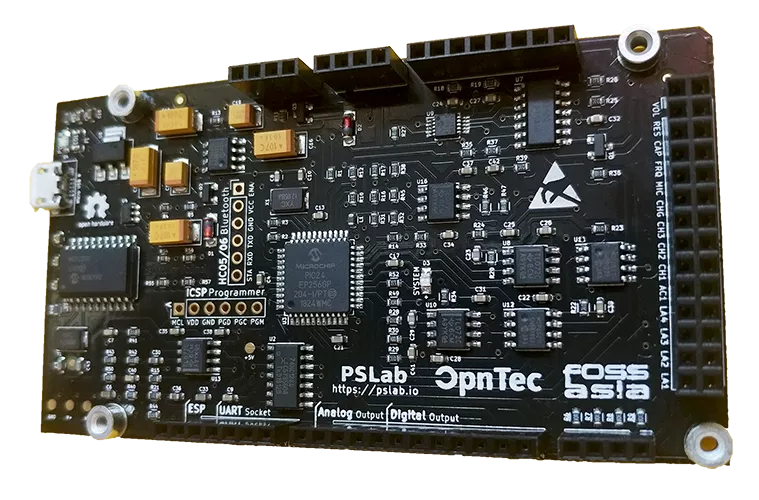
\includegraphics[scale=0.2]{pslab.png}
    \caption{Pocket Science Lab device}
    \label{fig:pslab}
\end{figure}

The application consists of two tasks. The first task set a GPIO up, wait for 1ms then set the same GPIO down. The other task do the same but an other GPIO. Using the collaborative scheduling, each task run after the other.

To use the collaborative scheduling, Contiki was used to run the application.

Using the Pocket Science Lab device, we were able to measure the voltage of the two GPIO used by the application. In the Fig.\ref{fig:ref}, we can see each GPIO being up and down for 1ms. We can also see during a small amount of time that none of the GPIO are up. The context switching happens during this period. No task is in the foreground during this time.


\begin{figure}[!h]
    \centering
    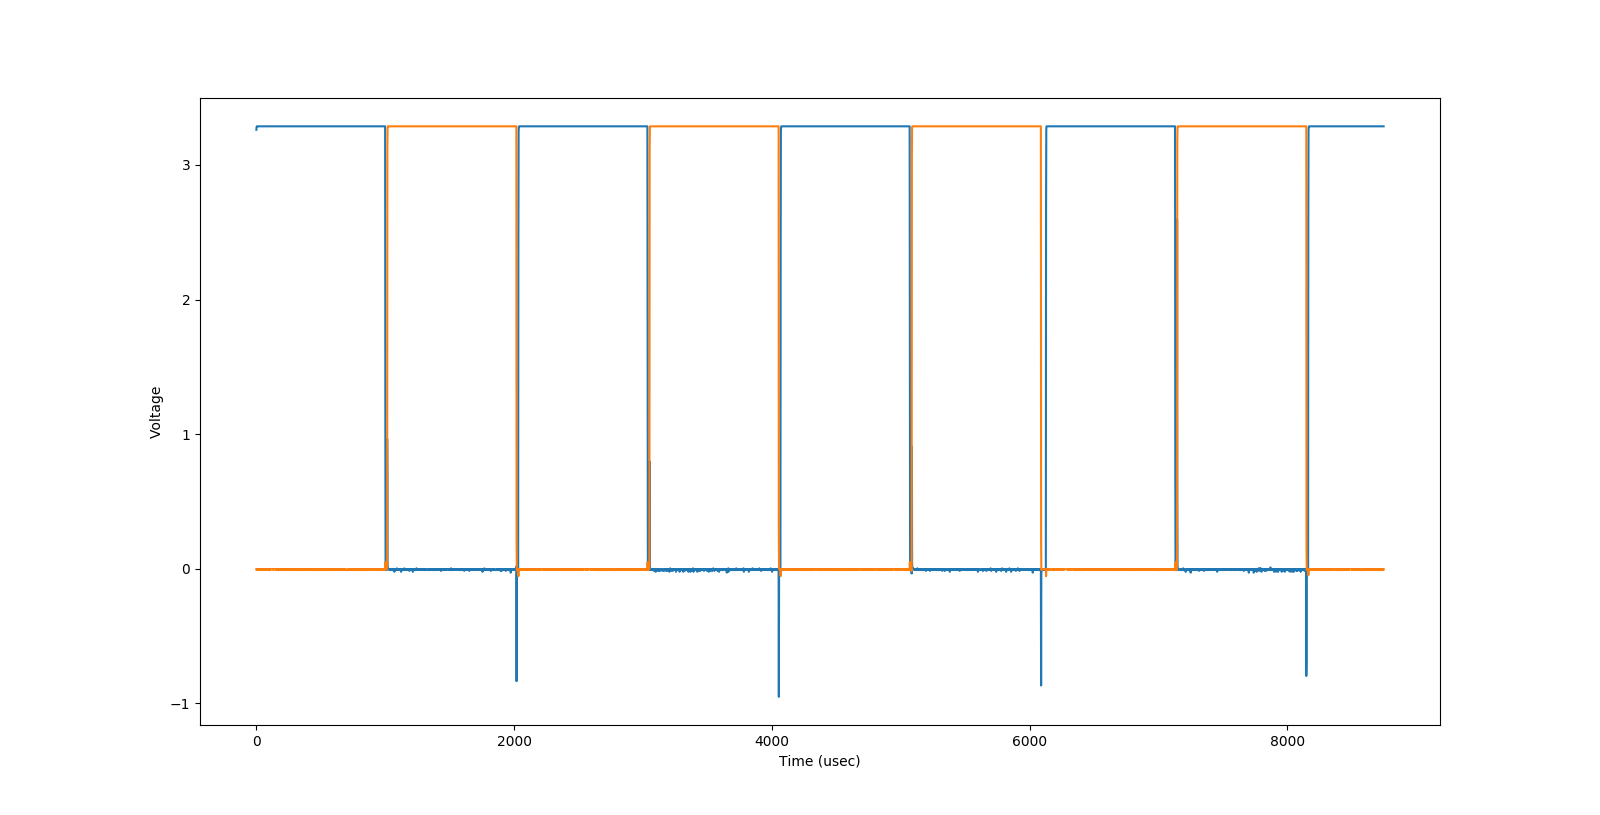
\includegraphics[scale=0.2]{ref.png}
    \caption{Reference measurement made with PSLab}
    \label{fig:ref}
\end{figure}



Using this reference, we can see how our framework change the performance of the application. Ideally, the time between two tasks should not change with our framework.

\section{EMBEDDED FRAMEWORK OVERHEAD}

Using the Pocket Science Lab device, we did the same experience describe in section \ref{sec:ref}. Fig.\ref{fig:framework_overhead} shows the results of the experiment.

\begin{figure}[!h]
    \centering
    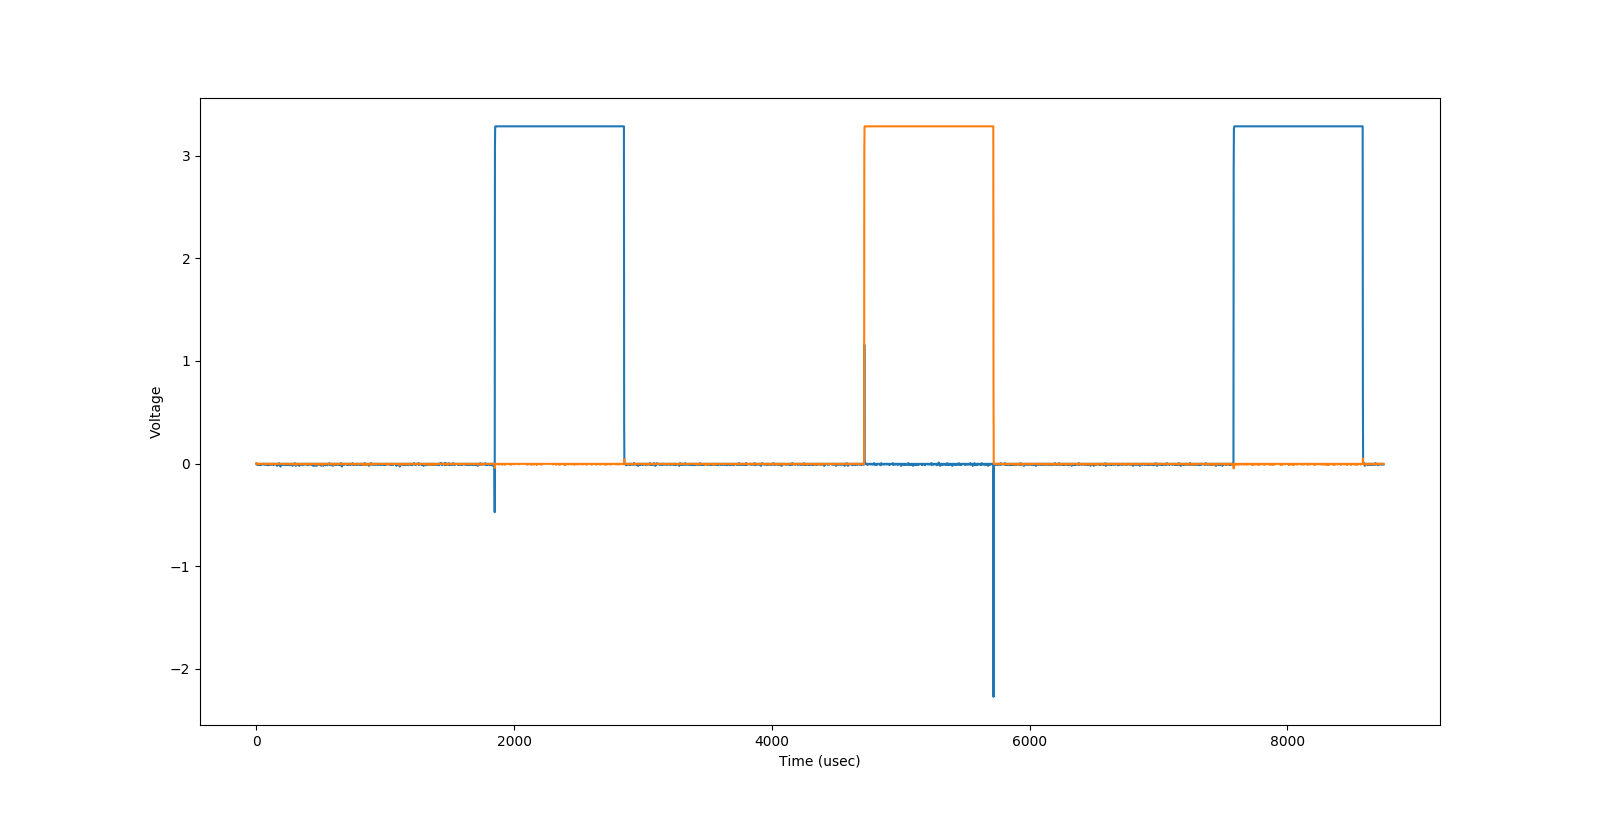
\includegraphics[scale=0.2]{framework_overhead.png}
    \caption{Embedded Framework Overhead measured with PSLab}
    \label{fig:framework_overhead}
\end{figure}

Table \ref{table:context_switching_times} compares the context switching time with and without our benchmarking framework. We can see that the framework add a huge overhead.


\begin{table}[!h]
    \centering
    \caption{Context switching times measured with the Pocket Science Lab device}
    \begin{tabular}{llll}
        \cline{2-4}
        & Mean ($\mu s$) & Median ($\mu s$) & Mode ($\mu s$) \\ \cline{2-4}
        Without the framework & 18.47 & 15.75 & 15.75 \\
        With the framework & 1864.33 & 1863.75 & 1863.75
    \end{tabular}
    \label{table:context_switching_times}
\end{table}

\section{PYTHON ALTERNATIVE}

    


\section{CONCLUSION}


\addtolength{\textheight}{-12cm}   % This command serves to balance the column lengths
                                  % on the last page of the document manually. It shortens
                                  % the textheight of the last page by a suitable amount.
                                  % This command does not take effect until the next page
                                  % so it should come on the page before the last. Make
                                  % sure that you do not shorten the textheight too much.

%%%%%%%%%%%%%%%%%%%%%%%%%%%%%%%%%%%%%%%%%%%%%%%%%%%%%%%%%%%%%%%%%%%%%%%%%%%%%%%%



%%%%%%%%%%%%%%%%%%%%%%%%%%%%%%%%%%%%%%%%%%%%%%%%%%%%%%%%%%%%%%%%%%%%%%%%%%%%%%%%



%%%%%%%%%%%%%%%%%%%%%%%%%%%%%%%%%%%%%%%%%%%%%%%%%%%%%%%%%%%%%%%%%%%%%%%%%%%%%%%%


%%%%%%%%%%%%%%%%%%%%%%%%%%%%%%%%%%%%%%%%%%%%%%%%%%%%%%%%%%%%%%%%%%%%%%%%%%%%%%%%

\end{document}
